\documentclass{article}
\usepackage[T1]{fontenc}
\usepackage{lmodern}
\usepackage{graphicx}
\usepackage{amsmath,amssymb}
\usepackage[a4paper,margin=2cm]{geometry}
\usepackage[absolute,overlay]{textpos}
\setlength{\TPHorizModule}{1mm}
\setlength{\TPVertModule}{1mm}
\usepackage[indonesian]{babel}
\usepackage{hyperref}
\setlength{\emergencystretch}{2em}
% unit: Halaman 97

\begin{document}

% === Halaman 97 (llm) ===

\begin{itemize}
  \item Contoh:
\end{itemize}

\vspace{10mm}

\[ K = \begin{pmatrix} 17 & 17 & 5 \\ 21 & 18 & 21 \\ 2 & 2 & 19 \end{pmatrix} \]

Plainteks: \texttt{paymoremoney} \\
Enkripsi tiga huruf pertama: $\text{pay} = (15, 0, 24)$

\vspace{10mm}

\[ C = \begin{pmatrix} 17 & 17 & 5 \\ 21 & 18 & 21 \\ 2 & 2 & 19 \end{pmatrix} \begin{pmatrix} 15 \\ 0 \\ 24 \end{pmatrix} = \begin{pmatrix} 375 \\ 819 \\ 486 \end{pmatrix} \pmod{26} = \begin{pmatrix} 11 \\ 13 \\ 18 \end{pmatrix} = \text{LNS} \]

Cipherteks selengkapnya: \texttt{LNSHDLEWMTRW}

% deskripsi: Tabel pemetaan huruf alfabet A-Z ke angka 0-25
% bbox normalisasi: [0.0600, 0.1080, 0.9400, 0.9120]
\begin{textblock*}{184.80mm}(12.60mm,32.08mm)
\noindent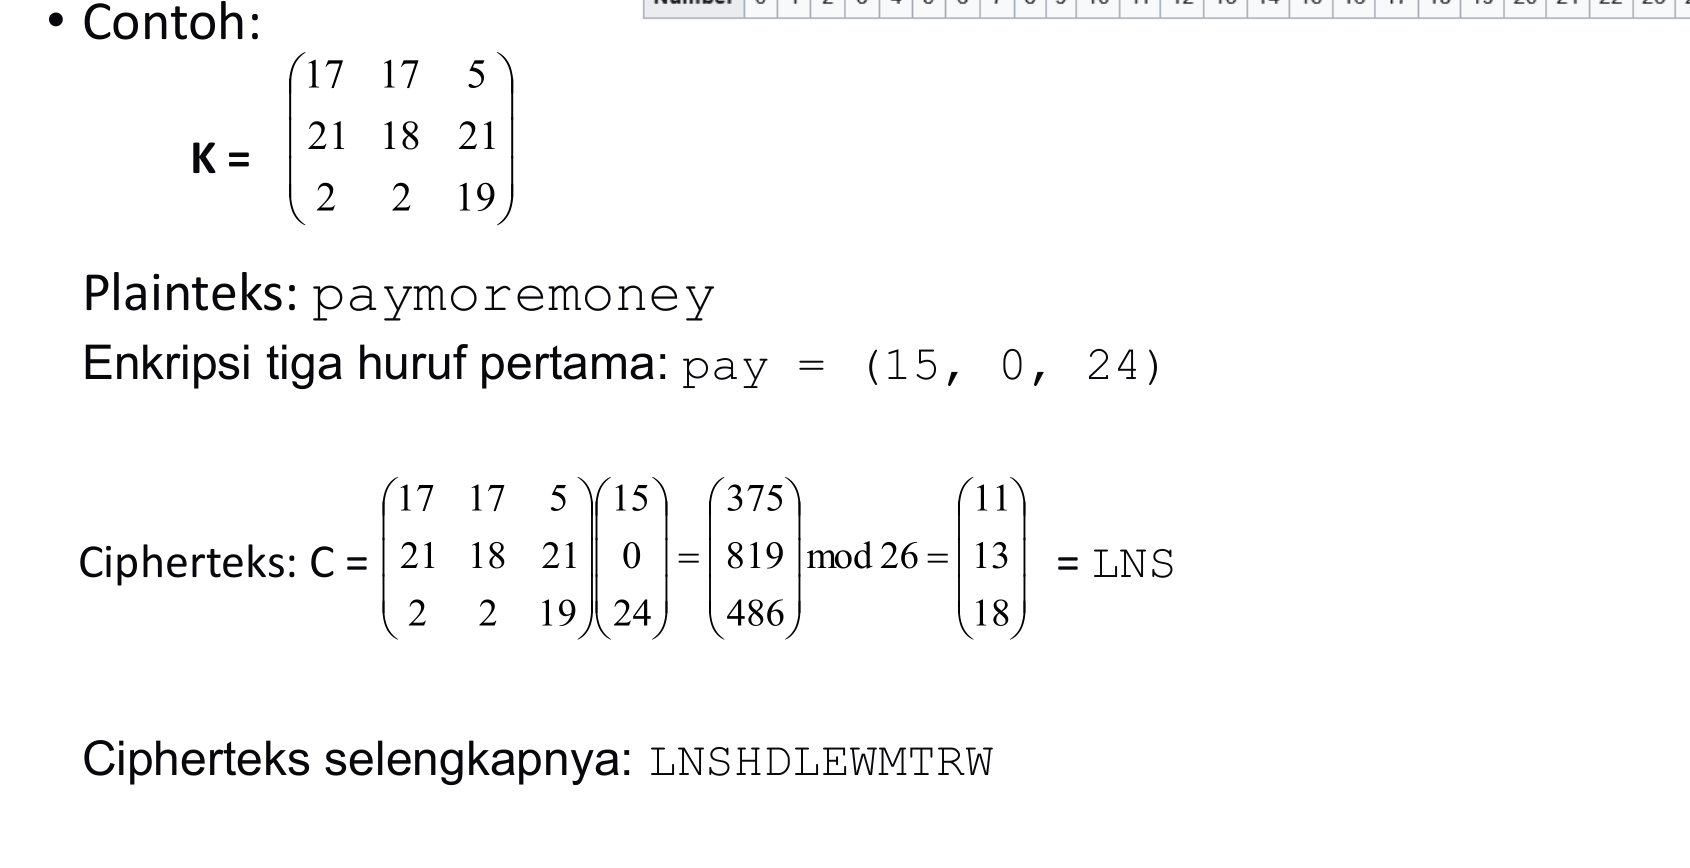
\includegraphics[width=184.80mm,height=238.79mm]{../../images/llm/page_097_img_01.png}%
\end{textblock*}

% bbox perkiraan otomatis: Tabel pemetaan huruf alfabet A-Z ke angka 0-25

\end{document}
